\begin{landscape}
\section{Complete kernel-matching follow-up}\label{app:kernel-matching}
All values below are endpoint means $\pm$ sample SD across ten blocks.
The nearest and one-to-one scores use signed cosines. Coverage counts
nearest-template identities, not independent semantic concepts. The analysis
uses only saved Stage B checkpoints; no spectrum or frozen conditions from
Stage A were added. These descriptive comparisons are exploratory.

{\small
\setlength{\tabcolsep}{3pt}
\begin{longtable}{p{.28\linewidth}p{.24\linewidth}rrr}
\caption{All endpoint kernel-matching means.}\\
\toprule
Setting & Condition & Nearest & One-to-one & Coverage \\
\midrule
\endhead
\bottomrule
\endlastfoot
single\_\allowbreak shape / TinyCNN & random & 0.300 $\pm$ 0.023 & 0.267 $\pm$ 0.033 & 9.700 $\pm$ 1.703 \\
single\_\allowbreak shape / TinyCNN & random\_\allowbreak unitnorm & 0.288 $\pm$ 0.022 & 0.256 $\pm$ 0.034 & 9.700 $\pm$ 1.703 \\
single\_\allowbreak shape / TinyCNN & template\_\allowbreak init & 0.610 $\pm$ 0.021 & 0.605 $\pm$ 0.021 & 13.300 $\pm$ 1.337 \\
single\_\allowbreak shape / TinyCNN & template\_\allowbreak release & 0.690 $\pm$ 0.017 & 0.686 $\pm$ 0.017 & 14.200 $\pm$ 1.033 \\
single\_\allowbreak shape / TinyCNN & template\_\allowbreak retention\_\allowbreak 1 & 0.959 $\pm$ 0.003 & 0.959 $\pm$ 0.003 & 16.000 $\pm$ 0.000 \\
single\_\allowbreak shape / TwoLayerCNN & random & 0.261 $\pm$ 0.037 & 0.230 $\pm$ 0.039 & 9.200 $\pm$ 1.317 \\
single\_\allowbreak shape / TwoLayerCNN & random\_\allowbreak unitnorm & 0.228 $\pm$ 0.033 & 0.195 $\pm$ 0.039 & 8.300 $\pm$ 1.889 \\
single\_\allowbreak shape / TwoLayerCNN & template\_\allowbreak init & 0.799 $\pm$ 0.015 & 0.799 $\pm$ 0.015 & 15.700 $\pm$ 0.483 \\
single\_\allowbreak shape / TwoLayerCNN & template\_\allowbreak release & 0.942 $\pm$ 0.006 & 0.942 $\pm$ 0.006 & 16.000 $\pm$ 0.000 \\
single\_\allowbreak shape / TwoLayerCNN & template\_\allowbreak retention\_\allowbreak 1 & 1.000 $\pm$ 0.000 & 1.000 $\pm$ 0.000 & 16.000 $\pm$ 0.000 \\
two\_\allowbreak concepts / TinyCNN & random & 0.232 $\pm$ 0.034 & 0.199 $\pm$ 0.035 & 9.100 $\pm$ 1.524 \\
two\_\allowbreak concepts / TinyCNN & random\_\allowbreak unitnorm & 0.222 $\pm$ 0.031 & 0.191 $\pm$ 0.037 & 9.200 $\pm$ 1.398 \\
two\_\allowbreak concepts / TinyCNN & template\_\allowbreak init & 0.507 $\pm$ 0.022 & 0.496 $\pm$ 0.022 & 12.000 $\pm$ 1.054 \\
two\_\allowbreak concepts / TinyCNN & template\_\allowbreak release & 0.580 $\pm$ 0.011 & 0.574 $\pm$ 0.010 & 12.900 $\pm$ 0.994 \\
two\_\allowbreak concepts / TinyCNN & template\_\allowbreak retention\_\allowbreak 1 & 0.947 $\pm$ 0.004 & 0.947 $\pm$ 0.004 & 16.000 $\pm$ 0.000 \\
two\_\allowbreak concepts / TwoLayerCNN & random & 0.255 $\pm$ 0.027 & 0.231 $\pm$ 0.024 & 9.600 $\pm$ 1.075 \\
two\_\allowbreak concepts / TwoLayerCNN & random\_\allowbreak unitnorm & 0.243 $\pm$ 0.028 & 0.218 $\pm$ 0.027 & 9.000 $\pm$ 1.054 \\
two\_\allowbreak concepts / TwoLayerCNN & template\_\allowbreak init & 0.746 $\pm$ 0.017 & 0.746 $\pm$ 0.017 & 15.400 $\pm$ 0.699 \\
two\_\allowbreak concepts / TwoLayerCNN & template\_\allowbreak release & 0.907 $\pm$ 0.012 & 0.907 $\pm$ 0.012 & 16.000 $\pm$ 0.000 \\
two\_\allowbreak concepts / TwoLayerCNN & template\_\allowbreak retention\_\allowbreak 1 & 0.999 $\pm$ 0.000 & 0.999 $\pm$ 0.000 & 16.000 $\pm$ 0.000 \\
\end{longtable}}

\end{landscape}

\begin{figure}[p]
\centering
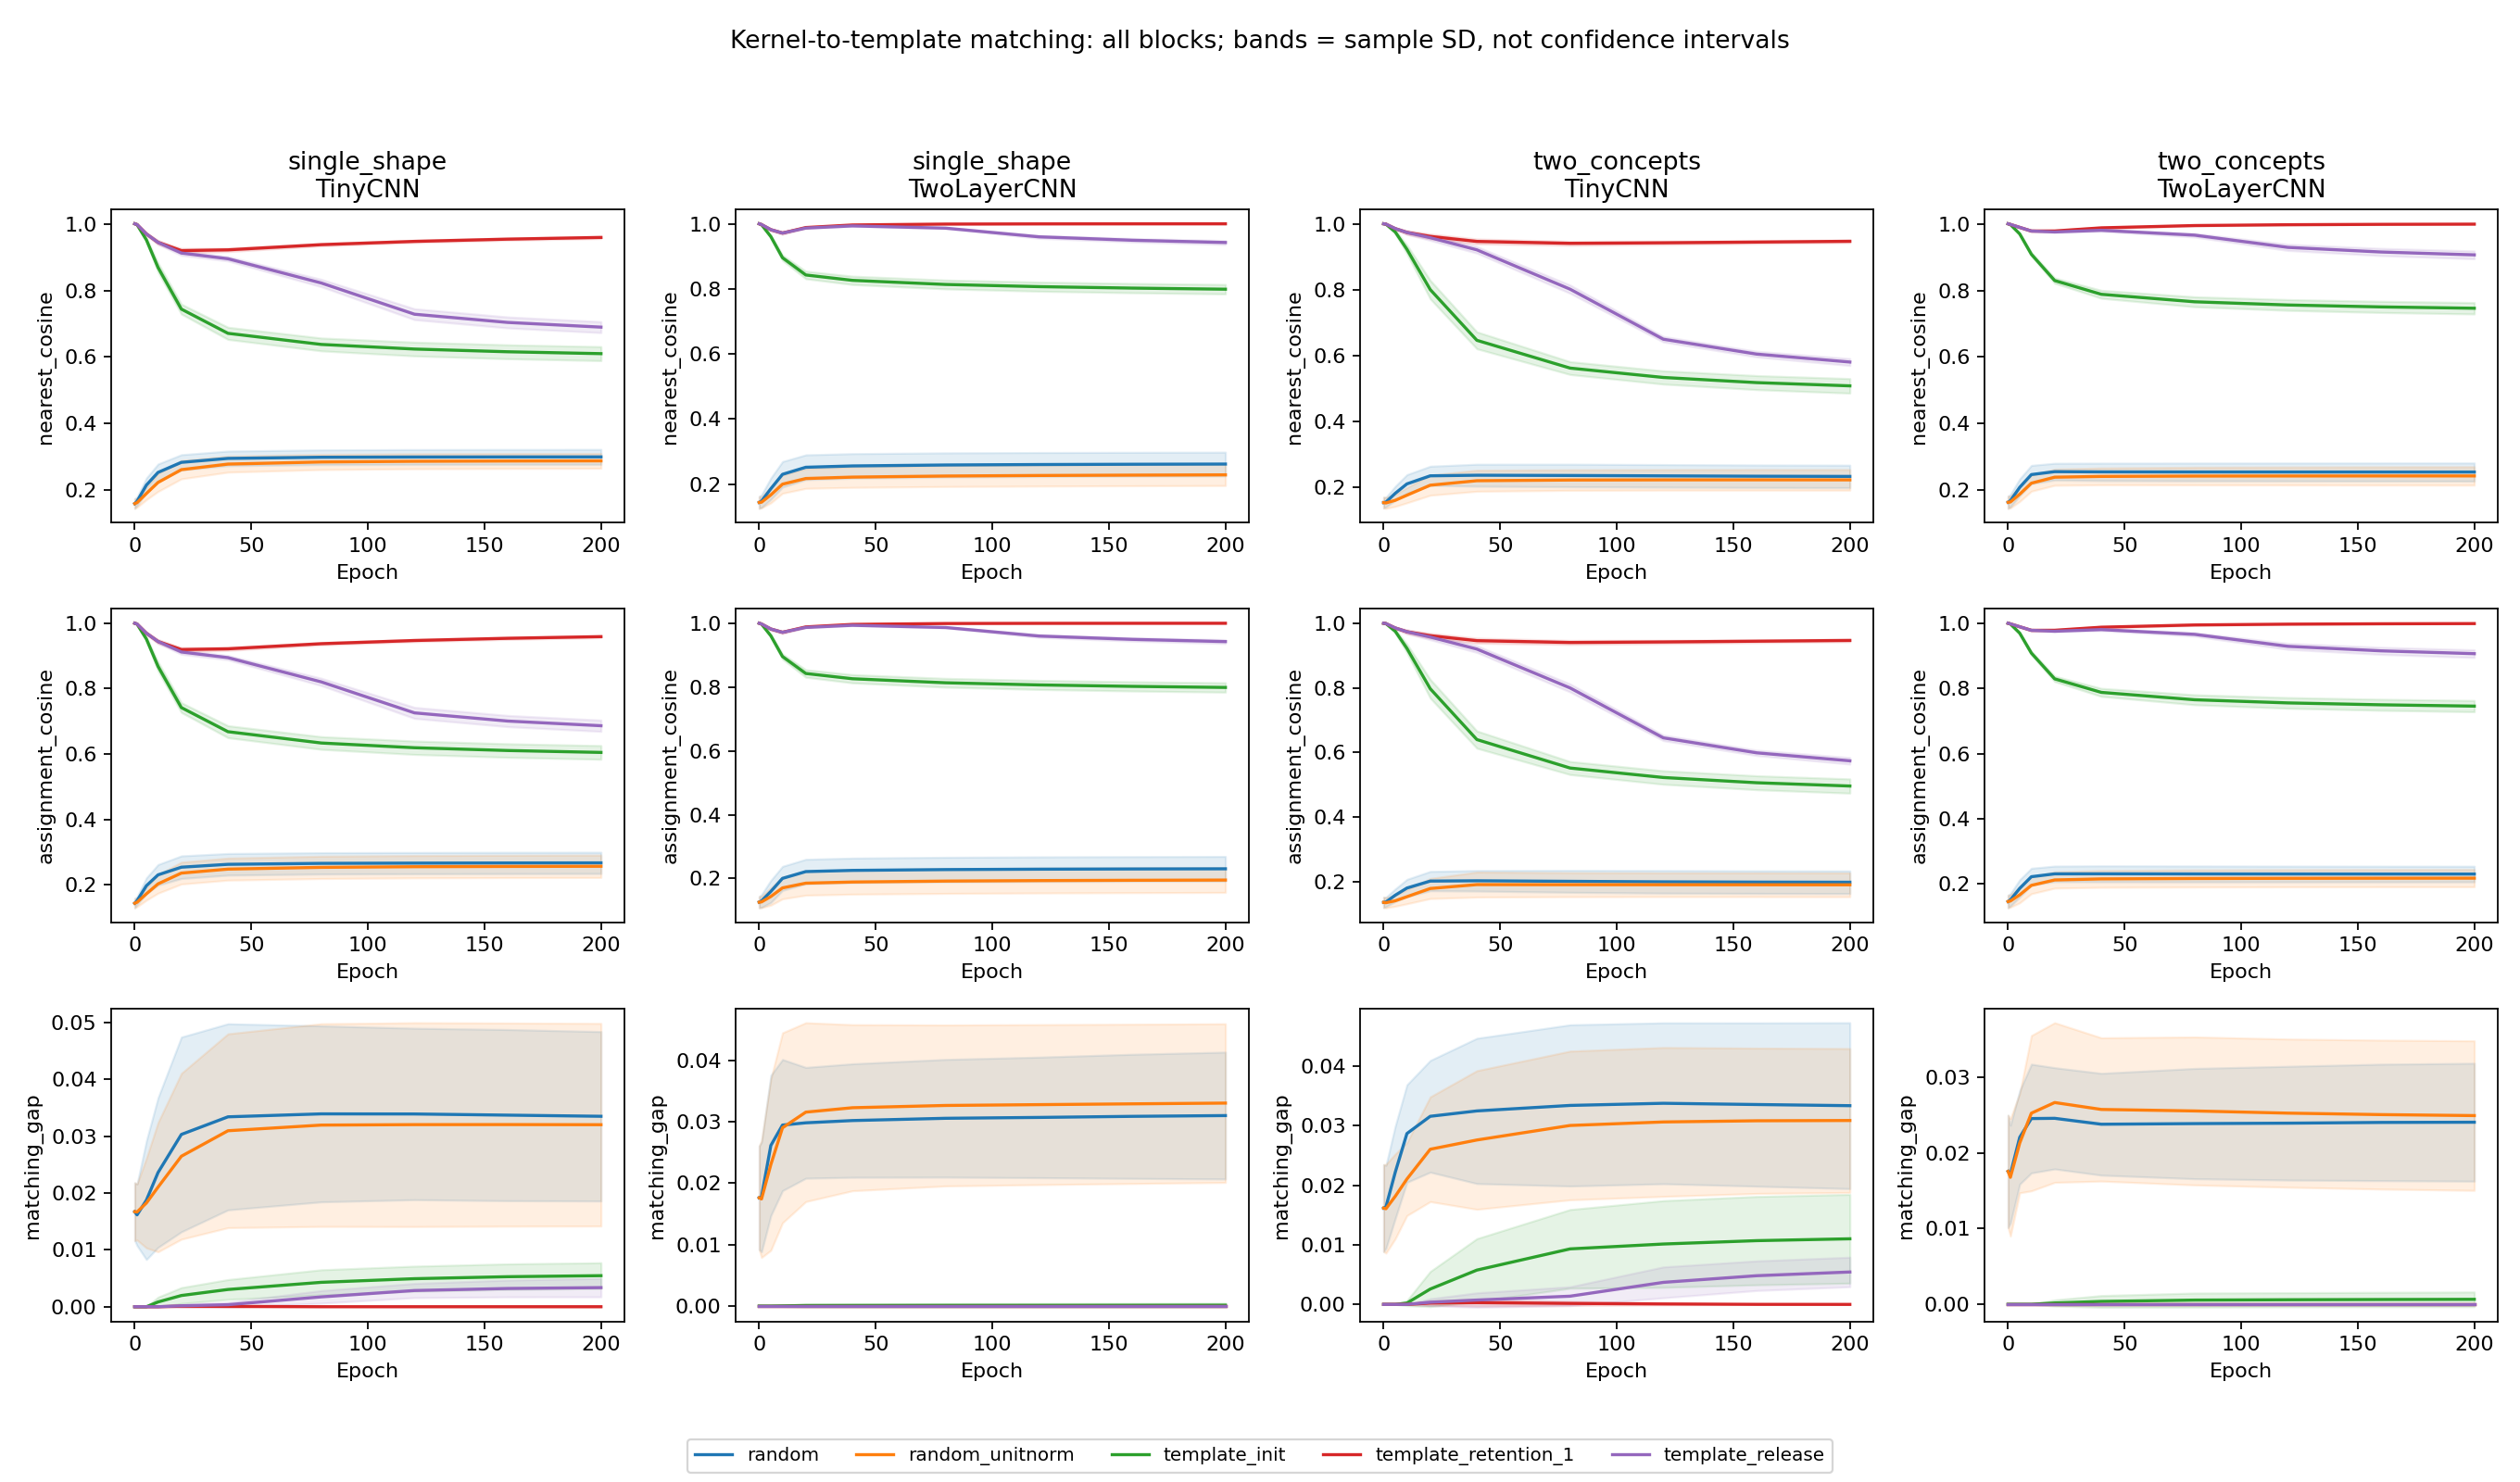
\includegraphics[width=\linewidth]{../analysis/kernel_similarity/results/matching_trajectories.png}
\caption{Nearest-template alignment, maximum-weight one-to-one alignment, and
their gap over all saved epochs. All five conditions and four settings are
shown. Bands are sample SD over ten blocks, not confidence intervals.}
\end{figure}
\begin{figure}[p]
\centering
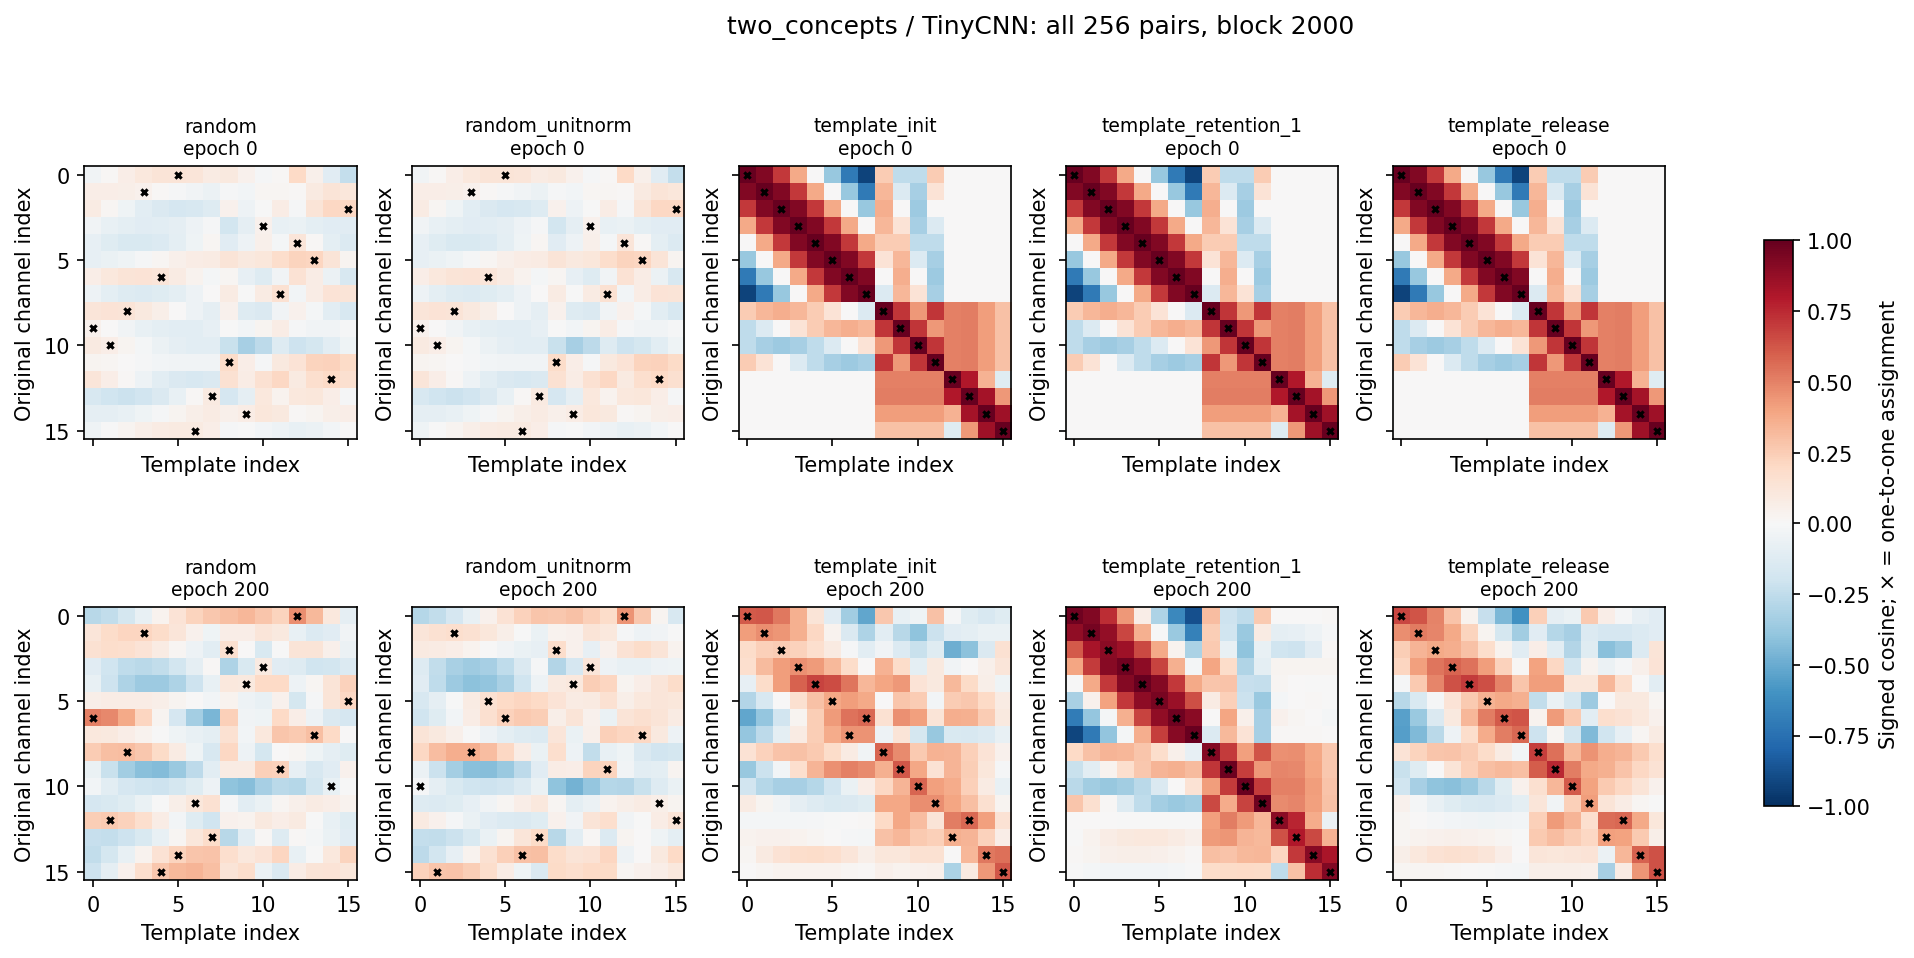
\includegraphics[width=\linewidth]{../analysis/kernel_similarity/results/matrices_two_concepts_TinyCNN.png}
\caption{All 256 signed kernel/template similarities for each condition at
initialization and epoch 200, two\_concepts/TinyCNN, fixed block 2000.
Rows retain original channel indices, columns retain template indices;
black crosses mark the optimal one-to-one assignment. Values range from
$-1$ to $1$. Matrices and galleries for all settings are retained in the
derived analysis artifacts.}
\end{figure}
